% Drawing 154/06-13 -- folder 154, batch 06, archive page 116 (PDF page 117).
% Transcription: sur une feuille de listing imprimée (bannière de travail), des dessins en couleur : à droite, une droite vert clair coupée de quatre paires de droites orange, les arcs $a$, $b$, $b'$ marqués, des hachures ; en bas à gauche, un carré vert clair (côtés marqués $(1)$, $(2)$, $(3)$) aux coins duquel partent des arêtes vert foncé et des arcs orange marqués $\lambda$, $\mu$, $\lambda'$, $\mu'$ ; au milieu, un croquis au crayon d'un triangle avec les mêmes lettres ; à droite, le même carré, ses quatre côtés marqués $\mathrm{I}$, $\mathrm{II}$, $\mathrm{III}$, $\mathrm{IV}$, rempli d'arcs orange et de flèches, avec les lettres $a$, $b$, $a'$, $b'$, $\lambda$, $\mu$, $x$ et trois points d'interrogation
% Kind: line cut by four pairs of crossings; square with edges and arcs at the corners (two versions); pencil triangle. Method 2 (schematic redraw from the facsimile). Status: partial.
% Notes: On a printed listing (CRAY2 job banner and notice, 17 Aug 82; not reproduced). Right: a light green line cut by four pairs of orange lines, the arcs a, b, b' marked (only b' placed), pencil hatching (left out). Bottom left: a light green square (sides marked (1), (2), (3)) from whose corners leave dark green edges and orange arcs marked lambda, mu, lambda', mu' (labels placed at the corners). In the middle, a pencil sketch of a triangle with the same letters. Right: the same square, its four sides marked I, II, III, IV, filled with orange arcs and arrows, with the letters a, b, a', b', lambda, mu, x and three question marks (only the Roman numerals and the question marks are placed). The pencil strokes at the top of the sheet are not covered. Read from the page view. Still differs from the facsimile: On a printed listing (CRAY2 job banner and notice, 17 Aug 82; not reproduced). Right: a light green line cut by four pairs of orange lines, the arcs a, b, b' marked (only b' placed), pencil hatching (left out). The pencil strokes at the top of the sheet are not covered. 1 coloured or hatched triangle(s) are placed schematically and are not bounded by the strands that bound them on the page.
% Coordinates: 1 unit = 1 mm = 1/100 of the crop width (bbox in page fractions: [0.175, 0.137, 0.937, 0.528]).
% Redrawn by Claude (claude-opus-5-5), issue #73, 2026-11-07; not checked by a human; not compiled (no TeX in the session).
% Revised by Claude (claude-opus-5-5) 2026-11-09 (issue #128) after Michel's check: vertices snapped to exact intersections (drawn points on their lines, meeting ends on the stroke they meet, near-concurrent lines through one computed point, curve ends on their rim); labels at \small as in folder 80 batch 3. Status: partial.
% Rights: reproduces part of the work -- behind RENDER_TRANSCRIPTS, never published by itself.
\documentclass[tikz,border=3pt]{standalone}
\usepackage{amsmath,amssymb}
\usetikzlibrary{patterns,arrows.meta}
\tikzset{Or/.style={orange!90!black}, Ye/.style={yellow!80!orange}, Lg/.style={green!60!black!70}, Dg/.style={green!45!black}, Br/.style={brown!80!black}, Rd/.style={red!85!black}, Bl/.style={blue!70!black}, Gy/.style={black!40}, pencil/.style={black!45}, struck/.style={black!35}, mark/.style={circle,draw,inner sep=1.3pt}, pt/.style={circle,fill,inner sep=0.9pt}, opt/.style={circle,draw,fill=white,inner sep=1.1pt}}
\begin{document}
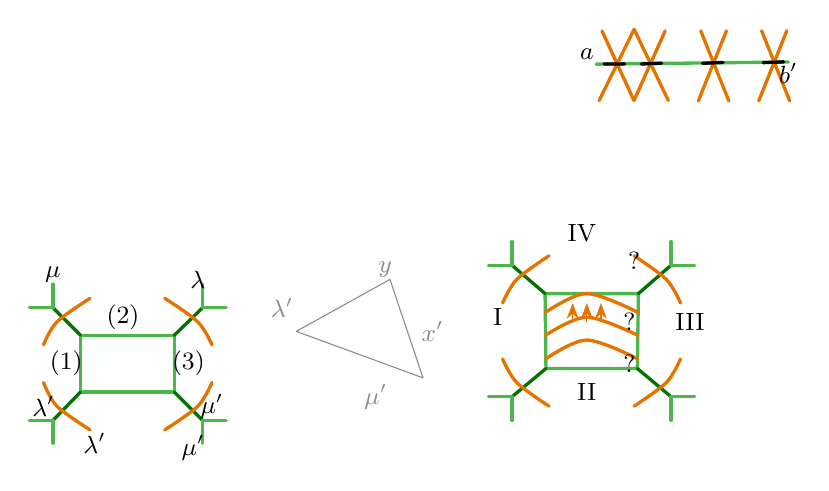
\begin{tikzpicture}[x=1mm,y=1mm,line cap=round,line join=round,font=\scriptsize]
\draw[Lg,very thick] (75,-22.06) -- (99.41,-21.79);
\draw[Or,very thick] (75.73,-17.84) -- (79.79,-26.69);
\draw[Or,very thick] (79.81,-17.64) -- (75.36,-26.69);
\draw[Or,very thick] (79.81,-17.64) -- (84.15,-26.68);
\draw[Or,very thick] (83.75,-17.83) -- (79.79,-26.69);
\draw[Or,very thick] (88.27,-17.83) -- (91.84,-26.74);
\draw[Or,very thick] (91.53,-17.83) -- (87.96,-26.74);
\draw[Or,very thick] (96,-17.82) -- (99.57,-26.73);
\draw[Or,very thick] (99.2,-17.82) -- (95.63,-26.73);
\draw[very thick] (76,-22.04) -- (78.61,-22.03);
\draw[very thick] (80.71,-22.04) -- (83.3,-21.93);
\draw[very thick] (88.5,-21.95) -- (91.1,-21.85);
\draw[very thick] (96.2,-21.87) -- (98.8,-21.77);
\node[inner sep=1pt] at (99.4,-23.2) {\small $b'$};
\node[inner sep=1pt] at (73.8,-20.8) {\small $a$};
\draw[Lg,very thick] (9.5,-56.5) -- (21.4,-56.5) -- (21.4,-63.7) -- (9.5,-63.7) -- cycle;
\draw[Dg,very thick] (9.5,-56.5) -- (6,-53);
\draw[Or,very thick] plot[smooth, tension=0.55] coordinates {(4.8,-57.7) (6.5,-54.8) (10.7,-51.8)};
\draw[Lg,very thick] (6,-53) -- (3,-53);
\draw[Lg,very thick] (6,-53) -- (6,-50);
\draw[Dg,very thick] (21.4,-56.5) -- (25,-53);
\draw[Or,very thick] plot[smooth, tension=0.55] coordinates {(26.2,-57.7) (24.4,-54.8) (20.2,-51.8)};
\draw[Lg,very thick] (25,-53) -- (28,-53);
\draw[Lg,very thick] (25,-53) -- (25,-50);
\draw[Dg,very thick] (21.4,-63.7) -- (25,-67.3);
\draw[Or,very thick] plot[smooth, tension=0.55] coordinates {(26.2,-62.5) (24.4,-65.5) (20.2,-68.5)};
\draw[Lg,very thick] (25,-67.3) -- (28,-67.3);
\draw[Lg,very thick] (25,-67.3) -- (25,-70.2);
\draw[Dg,very thick] (9.5,-63.7) -- (6,-67.3);
\draw[Or,very thick] plot[smooth, tension=0.55] coordinates {(4.8,-62.5) (6.5,-65.5) (10.7,-68.5)};
\draw[Lg,very thick] (6,-67.3) -- (3,-67.3);
\draw[Lg,very thick] (6,-67.3) -- (6,-70.2);
\node[inner sep=1pt] at (7.7,-60.1) {\small $(1)$};
\node[inner sep=1pt] at (14.9,-54.2) {\small $(2)$};
\node[inner sep=1pt] at (23.2,-60.1) {\small $(3)$};
\node[inner sep=1pt] at (6,-48.8) {\small $\mu$};
\node[inner sep=1pt] at (24.4,-49.4) {\small $\lambda$};
\node[inner sep=1pt] at (4.8,-65.5) {\small $\lambda'$};
\node[inner sep=1pt] at (26.2,-65.5) {\small $\mu'$};
\node[inner sep=1pt] at (11.3,-70.2) {\small $\lambda'$};
\node[inner sep=1pt] at (23.8,-70.8) {\small $\mu'$};
\draw[pencil] (36.9,-56) -- (48.8,-49.4) -- (53,-61.9) -- cycle;
\node[inner sep=1pt,pencil] at (35.1,-53) {\small $\lambda'$};
\node[inner sep=1pt,pencil] at (48.2,-48.2) {\small $y$};
\node[inner sep=1pt,pencil] at (54.2,-56) {\small $x'$};
\node[inner sep=1pt,pencil] at (47,-64.3) {\small $\mu'$};
\draw[Lg,very thick] (68.5,-51.2) -- (80.35,-51.2) -- (80.22,-60.72) -- (68.61,-60.72) -- cycle;
\draw[Dg,very thick] (68.5,-51.2) -- (64.3,-47.6);
\draw[Or,very thick] plot[smooth, tension=0.55] coordinates {(63.1,-52.4) (64.9,-49.4) (69,-46.4)};
\draw[Lg,very thick] (64.3,-47.6) -- (61.3,-47.6);
\draw[Lg,very thick] (64.3,-47.6) -- (64.3,-44.6);
\draw[Dg,very thick] (80.35,-51.2) -- (84.5,-47.6);
\draw[Or,very thick] plot[smooth, tension=0.55] coordinates {(85.7,-52.4) (83.9,-49.4) (79.8,-46.4)};
\draw[Lg,very thick] (84.5,-47.6) -- (87.5,-47.6);
\draw[Lg,very thick] (84.5,-47.6) -- (84.5,-44.6);
\draw[Dg,very thick] (80.22,-60.72) -- (84.5,-64.3);
\draw[Or,very thick] plot[smooth, tension=0.55] coordinates {(85.7,-59.5) (83.9,-62.5) (79.8,-65.5)};
\draw[Lg,very thick] (84.5,-64.3) -- (87.5,-64.3);
\draw[Lg,very thick] (84.5,-64.3) -- (84.5,-67.3);
\draw[Dg,very thick] (68.61,-60.72) -- (64.3,-64.3);
\draw[Or,very thick] plot[smooth, tension=0.55] coordinates {(63.1,-59.5) (64.9,-62.5) (69,-65.5)};
\draw[Lg,very thick] (64.3,-64.3) -- (61.3,-64.3);
\draw[Lg,very thick] (64.3,-64.3) -- (64.3,-67.3);
\draw[Or,very thick] plot[smooth, tension=0.55] coordinates {(68.53,-53.6) (73.8,-51.2) (80.32,-53.6)};
\draw[Or,very thick] plot[smooth, tension=0.55] coordinates {(68.56,-56.5) (73.8,-54.2) (80.28,-56.5)};
\draw[Or,very thick] plot[smooth, tension=0.55] coordinates {(68.6,-59.48) (73.8,-57.1) (80.24,-59.48)};
\draw[Or,-{Stealth[length=2mm]}] (72,-54.8) -- (72,-52.4);
\draw[Or,-{Stealth[length=2mm]}] (73.8,-54.8) -- (73.8,-52.4);
\draw[Or,-{Stealth[length=2mm]}] (75.6,-54.8) -- (75.6,-52.4);
\node[inner sep=1pt] at (73.2,-43.5) {\small $\mathrm{IV}$};
\node[inner sep=1pt] at (62.5,-54.2) {\small $\mathrm{I}$};
\node[inner sep=1pt] at (86.9,-54.8) {\small $\mathrm{III}$};
\node[inner sep=1pt] at (73.8,-63.7) {\small $\mathrm{II}$};
\node[inner sep=1pt] at (79.8,-47) {\small ?};
\node[inner sep=1pt] at (79.2,-54.8) {\small ?};
\node[inner sep=1pt] at (79.2,-60.1) {\small ?};
\end{tikzpicture}
\end{document}
